Il foglio di stile implementato garantisce un design fluido e scalabile, grazie all'utilizzo di unità di misura
sempre relative o in percentuale. \\Questo migliora l'accessibilità e garantisce una corretta visualizzazione delle pagine
su tutti i formati di schermi. \\Il sito dispone di 4 modalità di visualizzazione differente: desktop, tablet, mobile e di stampa.

\subsection{Desktop}
La versione desktop è stata pensata in modo da avere una navigazione estremamente semplice.\\ 
Nella colonna di sinistra sono presenti anche le news, con i relativi orari di apertura della pasticceria.\\ 
Da notare la larghezza massima impostata a 1200px, che permette agli utenti di utilizzare il sito con una finestra ridotta su schermi di certe dimensioni.

\begin{figure}[!h]
	\centering
	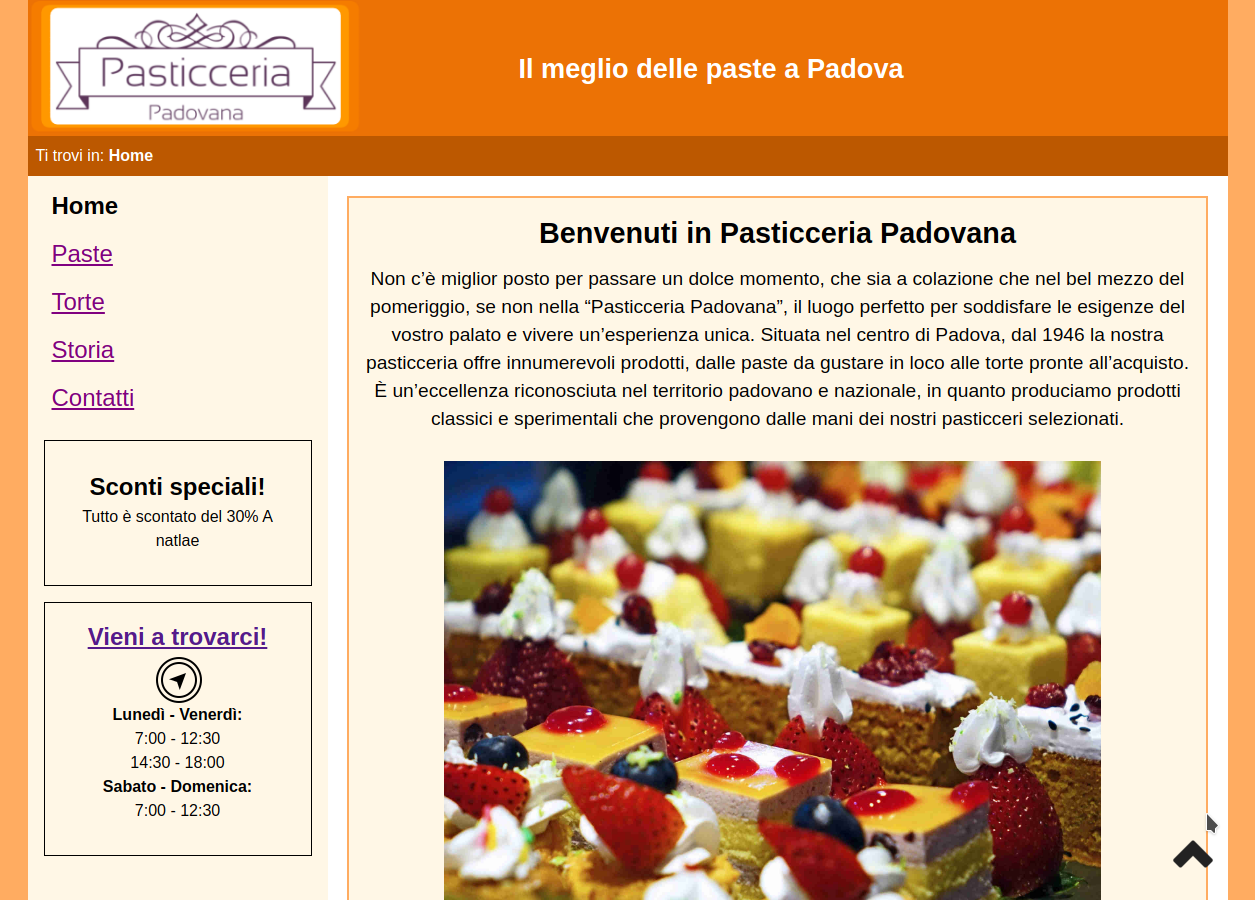
\includegraphics[width=1\linewidth]{sezioni/Progettazione/Immagini/desktop_example.png}
	\caption{Esempio di una pagina in versione desktop}
	\label{Fig:verDesktop}
\end{figure}
\newpage
\subsection{Tablet}
La versione tablet implementa l'interfaccia in modo diverso. Dato lo spazio limitato dello schermo, il gruppo ha deciso di implementare
un menù ad hamburger. Anche le news non sono più laterali, ma si trovano in cima al contenuto della pagina. In questo modo viene data
maggiore importanza alle news e agli orari della pasticceria, cosa necessaria nei dispositivi portatili.\\
Anche il form di login da parte dell'amministratore nelle versioni mobili è stato nascosto e reso disponibile tramite un bottone.
\begin{figure}[!h]		
    \centering		  
	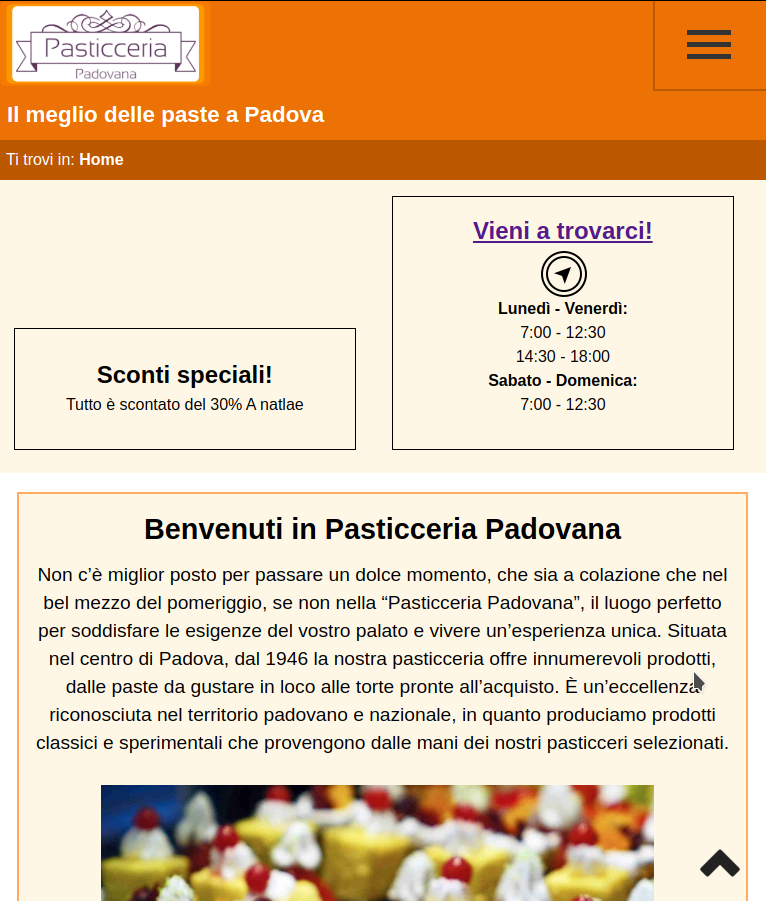
\includegraphics[width=0.8\linewidth]{sezioni/Progettazione/Immagini/tablet_example.png}
	\caption{Esempio di una pagina in versione tablet}
	\label{Fig:verTablet}
\end{figure}	    
\newpage

\subsection{Mobile}
La versione mobile differisce di molto poco rispetto alla versione tablet. Solo news e sezione vieni a trovarci con orari sono state poste incolonnate invece che affiancate.
\begin{figure}[!h]
    \centering		  
	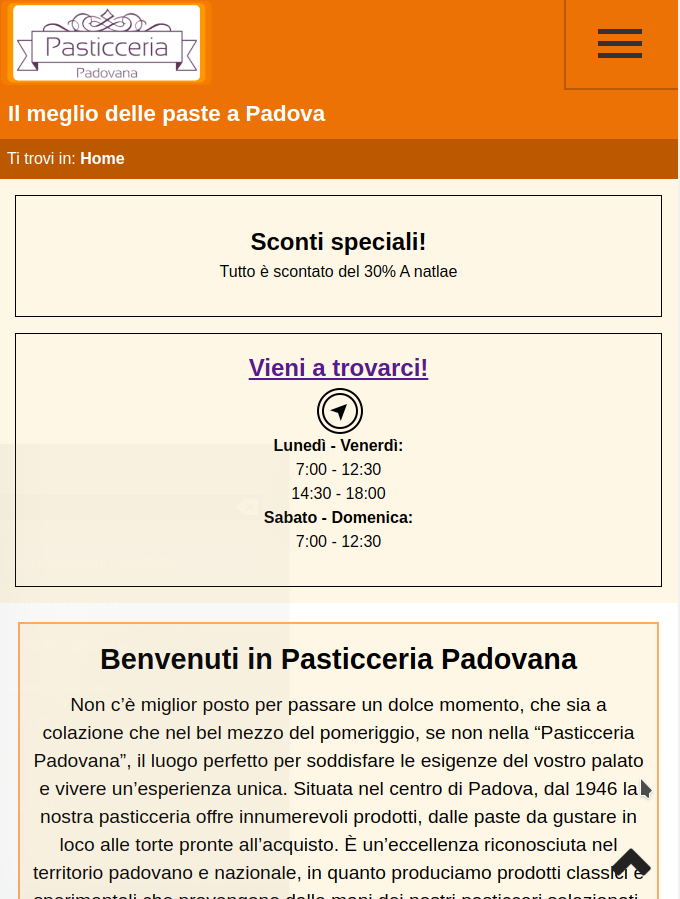
\includegraphics[width=0.8\linewidth]{sezioni/Progettazione/Immagini/mobile_example.png}
	\caption{Esempio di una pagina in versione mobile}
	\label{Fig:verMobile}
\end{figure}
\newpage

\subsection{Print}
La stampa elimina tutte le funzionalità interattive. In questo modo una pagina stampata conterrà solamente il contenuto interessato.\\
Vengono quindi eliminati la maggior parte degli stili, dei colori e delle immagini in quanto l'obbiettivo di una stampa è ottenere foglio 
contenente solo informazioni realmente utili.\\
La scelta è stata quella di mantenere le foto ai prodotti nella stampa. Questo poichè la presentazione dei prodotti di una pasticceria è di rilevante importanza.\\
\begin{figure}[!h]
    \centering		  
	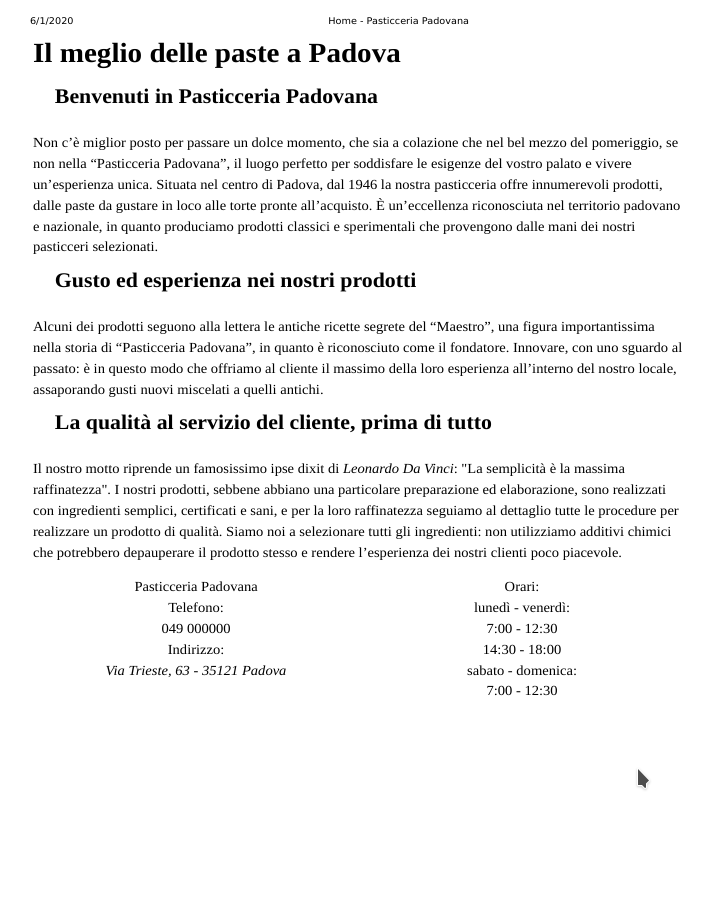
\includegraphics[width=0.8\linewidth]{sezioni/Progettazione/Immagini/print_example.png}
	\caption{Esempio di una stampa}
	\label{Fig:verPrint}
\end{figure}


\newpage